\subsection{Stakeholders}

The stakeholders of the project are individuals, organisations and societal groups which have interest in, and/or influence the project. The stakeholders along with their interaction with the project are depicted in Figure \ref{fig:stakeholder}. The relation of the stakeholders are listed in Table \ref{tab:sdl}. CASA regulate the operation of aircraft within Australia which directly effect the internal project development group. Other stakeholders include the honours team who will perform the research, design and assembly of the system. The intellectual property is owned by Lockheed Martin STELaRLab, with Dr Tim Payne and Dr Scott Beinke providing mentorship and in-kind support to the project. The university academic appointed to supervise the project is Dr Rey Chin. Other stakeholders include the University of Adelaide and Australian emergency fire services such as the CFS.


%\begin{figure}[H]
    %\centering
   % \includegraphics[width=1\textwidth]{stakeholderv2.jpg}
   % \caption{Stakeholder Diagram}
    %\label{fig:stakeholder}
%\end{figure}

\begin{figure}[H]
    \centering
    \usetikzlibrary{calc,positioning}
\resizebox{0.95\textwidth}{!}{
\tikzstyle{violet rectangle}=[rectangle,fill=purple!20,draw=violet,rounded corners,inner sep=15pt, ultra thick,minimum width=3cm, minimum height = 1.5cm]
\tikzstyle{grey rectangle}=[rectangle,fill=black!20,ultra thick,draw=black,rounded corners,minimum width=5cm, minimum height = 3cm]
\tikzstyle{orange line}=[line width=1.6pt]




\begin{tikzpicture}[remember picture,
  %simulator engine/.style={fill=black!10,rounded corners,inner sep=20pt},
 % topology/.style={rounded corners,draw=violet!50,fill=violet!20,thick},
  neuron/.style={fill=violet!10,draw=violet,rounded corners,inner sep=15pt, ultra thick},
  synapse/.style={draw=violet,fill=purple!20,rounded corners,inner sep=5pt},
  %empty synapse/.style={draw=violet!10,rounded corners,inner sep=5pt}
  ]
\node[violet rectangle] (1) at (10,10) {\textbf{Government}};
\node[violet rectangle] (2) at (10,20) {\textbf{Emergency Fire Service}};
\node[violet rectangle] (3) at (10,0) {\textbf{CASA}};

%\node[grey rectangle] (4) at (0,0) {Supply Chain}; 
%\node[grey rectangle] (5) at (0,10) {Honours Team}; 
%\node[grey rectangle] (6) at (0,20) {Operators};
%\node[grey rectangle] (7) at (20,0) {External};
%\node[grey rectangle] (8) at (20,10) {Internal};
%\node[grey rectangle] (9) at (20,20) {Observers};

\node at(10,10) {
    \begin{tikzpicture}
      \node[topology] (topology1) {
        \begin{tikzpicture}
         \node[neuron] (4) at (0,0) (4)  {
              \begin{tikzpicture}
                  \node [synapse,draw=violet] (synapse1-1-0) {$\text{External Manufacturing}$};
                  \node [synapse,draw=violet,below=0.1cm of synapse1-1-0] (synapse1-1-1) {$\text{External Part Suppliers}$};
                  %\node [synapse,draw=violet,below=0.1cm of synapse1-1-1] (synapse1-1-2) {$\text{Honours Supervisor}$};
              \end{tikzpicture}
          };
          \node[neuron] (5) at (0,10) (5)  {
              \begin{tikzpicture}
                  \node [synapse,draw=violet] (synapse1-1-0) {$\text{Internal Manufacturing}$};
                  \node [synapse,draw=violet,below=0.1cm of synapse1-1-0] (synapse1-1-1) {$\text{Designers and Engineers}$};
                  \node [synapse,draw=violet,below=0.1cm of synapse1-1-1] (synapse1-1-2) {$\text{Honours Supervisor}$};
              \end{tikzpicture}
          };
          
        \node[neuron] (6) at (0,20)  (6) {
              \begin{tikzpicture}
                  \node [synapse,draw=violet] (synapse1-2-0) {$\text{CFS Personnel}$};
                  \node [synapse,draw=violet,below=0.1cm of synapse1-2-0] (synapse1-2-1) {$\text{Maintenance Crews}$};
                  %\node [synapse,draw=violet,below=0.1cm of synapse1-2-1] (synapse1-2-2) {$\text{Synapse}_{2}$};
                  %\node [synapse,draw=violet,below=0.1cm of synapse1-2-2] (synapse1-2-3) {$\text{Synapse}_{3}$};
              \end{tikzpicture}
          };
          \node (7) at (20,0) [neuron] (7) {
              \begin{tikzpicture}
                  \node [synapse,draw=violet] (synapse1-3-0) {$\text{Lockheed Martin STELarLAB}$};
                  \node [synapse,draw=violet,below=0.1cm of synapse1-3-0] (synapse1-3-1) {$\text{Engineering Body of Knowledge}$};
                  %\node [synapse,draw=violet,below=0.1cm of synapse1-3-1] (synapse1-3-2) {$\text{Synapse}_{2}$};
                  %\node [synapse,draw=violet,below=0.1cm of synapse1-3-2] (synapse1-3-3) {$\text{Synapse}_{3}$};
              \end{tikzpicture}
          };
          \node (8) at (20,10) [neuron] (8) {
              \begin{tikzpicture}
                  \node [synapse,draw=violet] (synapse1-3-0) {$\text{The University of Adelaide}$};
                  \node [synapse,draw=violet,below=0.1cm of synapse1-3-0] (synapse1-3-1) {$\text{UofA Workshop Staff}$};
                  \node [synapse,draw=violet,below=0.1cm of synapse1-3-1] (synapse1-3-2) {$\text{URAF}$};
                  %\node [synapse,draw=violet,below=0.1cm of synapse1-3-2] (synapse1-3-3) {$\text{Synapse}_{3}$};
              \end{tikzpicture}
          };
          \node (9) at (20,20) [neuron] (9) {
              \begin{tikzpicture}
                  \node [synapse,draw=violet] (synapse1-3-0) {$\text{Communities at Risk}$};
                  \node [synapse,draw=violet,below=0.1cm of synapse1-3-0] (synapse1-3-1) {$\text{Wildlife}$};
                  %\node [synapse,draw=violet,below=0.1cm of synapse1-3-1] (synapse1-3-2) {$\text{Synapse}_{2}$};
                  %\node [synapse,draw=violet,below=0.1cm of synapse1-3-2] (synapse1-3-3) {$\text{Synapse}_{3}$};
              \end{tikzpicture}
          };

          \node [black,below] at (4.north)  {$\text{\textbf{Supply Chain}}$};
          \node [black,below] at (5.north)  {$\text{\textbf{Honours Team}}$};
          \node [black,below] at (6.north)  {$\text{\textbf{Operators}}$};
          \node [black,below] at (7.north)  {$\text{\textbf{External}}$};
          \node [black,below] at (8.north)  {$\text{\textbf{Internal}}$};
          \node [black,below] at (9.north)  {$\text{\textbf{Observers}}$};
        \end{tikzpicture}
      };

    \end{tikzpicture}
    };
 

\draw[<->,orange line] ($ (2) + (3,0) $) .. controls +(right:3cm) and +(left:3cm).. node[above,sloped] {\Large{a}} ($ (9) + (-3,0) $);
\draw[<->,orange line] ($ (2) + (-3,0) $) .. controls +(left:3cm) and +(right:3cm).. node[above,sloped] {\Large{b}} ($ (6) + (2.15,0) $);
\draw[->,orange line] ($ (9) + (-3,-1.) $) .. controls +(left:3cm) and +(right:3cm).. node[below right,sloped] {\Large{c}} ($(3)+(1.5,0.5)$);
\draw[->,orange line] ($(5)+(0,1.8)$) .. controls +(up:3cm) and +(down:3cm).. node[above,sloped] {\Large{d}} ($ (2) + (-1,-0.75) $);
\draw[<->,orange line] (1) .. controls +(up:1cm) and +(down:1cm).. node[above right,sloped] {\Large{e}} (2);
\draw[->,orange line] (1) .. controls +(down:1cm) and +(up:1cm).. node[above,sloped] {\Large{f}} (3);
\draw[->,orange line] ($(1)+(1.8,0)$) .. controls +(right:1cm) and +(left:2cm).. node[below,sloped] {\Large{g}} ($(8)+(-3.5,-0.5)$);
\draw[->,orange line] (3) .. controls +(left:4cm) and +(down:3cm).. node[above,sloped] {\Large{h}} (5);
\draw[->,orange line] (1) .. controls +(left:4cm) and +(right:5cm).. node[above left,sloped] {\Large{i}} ($(4)+(2.6,0)$);
\draw[->,orange line] (3) .. controls +(right:3) and +(down:3cm).. node[above right ,sloped] {\Large{j}} (8);
\draw[<->,orange line] ($ (5) + (1,1.8) $) .. controls +(up:4cm) and +(up:4cm).. node[below right,sloped] {\Large{k}} ($ (8) + (-1,1.8) $);
\draw[<->,orange line] ($ (5) + (-1,1.8) $) .. controls +(up:3cm) and +(down:3cm).. node[above ,sloped] {\Large{l}} (6);
\draw[<->,orange line] ($ (5) + (-1,-1.75) $) .. controls +(down:3cm) and +(up:3cm).. node[above,sloped] {\Large{m}} ($(4)+(0,1.4)$);
\draw[<->,orange line] (7) .. controls +(up:3cm) and +(down:3cm).. node[above right,sloped] {\Large{n}} ($ (5) + (1,-1.75) $);

\end{tikzpicture}
}
    \caption[Stakeholder Diagram]{Stakeholder Diagram depicting the key groups and individuals and their connection to the project}
    \label{fig:stakeholder}
\end{figure}

\begin{table}[H]
\centering
\caption{Legend for connections on the Stakeholder Diagram} 
\label{tab:sdl}
\resizebox{0.8\textwidth}{!}{%
\begin{tabular}{|l||l|l|l||l|}
\cline{1-2} \cline{4-5}
a & Sharing Data and Results &  & h & Restrictions \\ \cline{1-2} \cline{4-5} 
b & Instructions and Data &  & i & Restrictions \\ \cline{1-2} \cline{4-5} 
c & Influence &  & j & Restrictions and Influence \\ \cline{1-2} \cline{4-5} 
d & Instructions and Insight &  & k & Funding \\ \cline{1-2} \cline{4-5} 
e & Funding &  & l & Documentation and Feedback \\ \cline{1-2} \cline{4-5} 
f & Law and Legislation &  & m & Supply and Requests \\ \cline{1-2} \cline{4-5} 
g & Funding and Influence &  & n & Funding \\ \cline{1-2} \cline{4-5} 
\end{tabular}%
}
\end{table}

The stakeholder interest influence matrix, in Figure \ref{fig:stakeholdermatrix} depicts the relation between stakeholder project interest and stakeholder influence resulting in how they should be managed. Stakeholders with high interest and influence such as team members, the project supervisor and sponsors fall into the key stakeholder section of the matrix and are to be managed closely. The identified Key Stakeholders will have their inputs prioritised throughout the project. Stakeholders with high influence and low interest such as the Government and CASA need to be kept informed throughout the duration of the project to ensure compliance with appropriate regulations. Stakeholders with high interest and low influence include persons that the system effects such as those impacted by bushfires and need to be considered throughout the design process. 


\begin{figure}[H]
    \centering
    \begin{figure}
\centering
\begin{minipage}{.6\textwidth}
  \centering
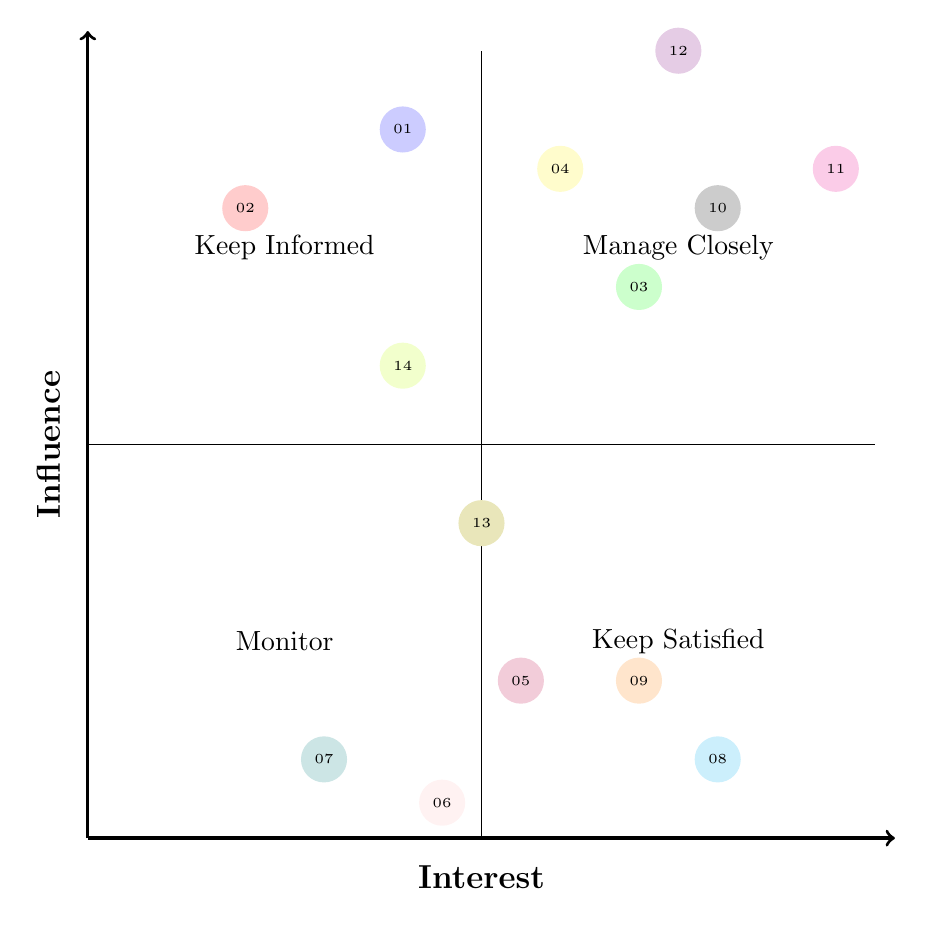
\begin{tikzpicture}
\draw [->,very thick] (0,0) --(0,10.25);
\draw [->,very thick] (0,0) --(10.25,0);
\draw (0,5) --(10,5);
\draw (5,0) --(5,10);

\node[circle,fill=blue!20] (CASA) at (4,9) {\tiny{01}};
\node[circle,fill=red!20] (Government) at (2,8) {\tiny{02}};
\node[circle,fill=green!20] (UofA) at (7,7) {\tiny{03}};
\node[circle,fill=yellow!20] (Emergency Fire Services) at (6,8.5) {\tiny{04}};
\node[circle,fill=purple!20] (Communities at Risk) at (5.5,2) {\tiny{05}};
\node[circle,fill=pink!20] (Wildlife) at (4.5,0.45) {\tiny{06}};
\node[circle,fill=teal!20] (Suppliers) at (3,1) {\tiny{07}};
\node[circle,fill=cyan!20] (External Manufacturers) at (8,1) {\tiny{08}};
\node[circle,fill=orange!20] (Maintenance Crews) at (7,2) {\tiny{09}};
\node[circle,fill=black!20] (Honours Supervisor) at (8,8) {\tiny{10}};
\node[circle,fill=magenta!20] (Honours Team Members) at (9.5,8.5) {\tiny{11}};
\node[circle,fill=violet!20] (Lockheed Martin STELarLAB) at (7.5,10) {\tiny{12}};
\node[circle,fill=olive!20] (UoA Workshop) at (5,4) {\tiny{13}};
\node[circle,fill=lime!20] (URAF) at (4,6) {\tiny{14}};

\node (a) at (2.5,2.5) {Monitor};
\node (b) at (2.5,7.5) {Keep Informed};
\node (c) at (7.5,2.5) {Keep Satisfied};
\node (d) at (7.5,7.5) {Manage Closely};

\node (e) at (5,- 0.5) {\textbf{\large{Interest}}};
\node[rotate=90] (f) at (-.5,5) {\textbf{\large{Influence}}};
%\node[rotate=90] at (0,5) {Influence}
\end{tikzpicture}   

\end{minipage}%
\begin{minipage}{.4\textwidth}
 \begin{flushright}
\resizebox{3.5cm}{!}{
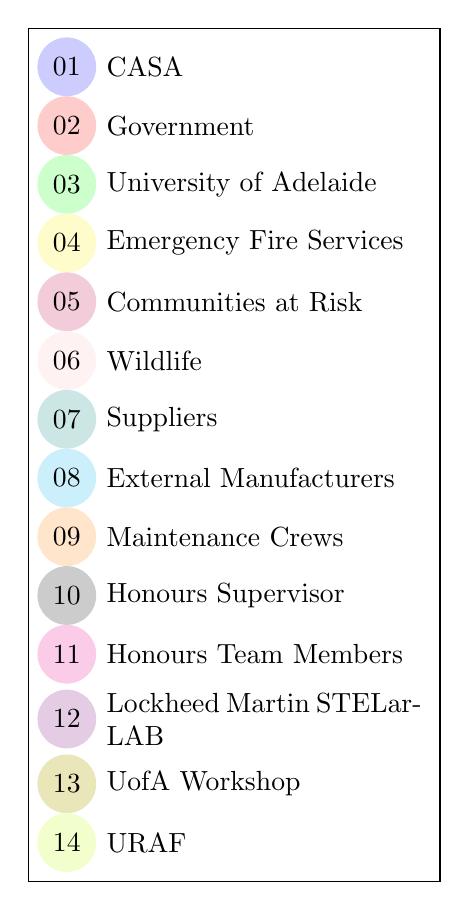
\begin{tikzpicture}
\matrix [draw,below right] at (11,10) {
  \node [circle,fill=blue!20,label=right:CASA] {01}; \\
  \node [circle,fill=red!20,label=right:Government] {02}; \\
  \node [circle,fill=green!20,label=right:University of Adelaide] {03}; \\
  \node [circle,fill=yellow!20,label=right:Emergency Fire Services] {04}; \\
  \node [circle,fill=purple!20,label=right:Communities at Risk] {05}; \\
  \node [circle,fill=pink!20,label=right:Wildlife] {06}; \\
  \node [circle,fill=teal!20,label=right:Suppliers] {07}; \\
  \node [circle,fill=cyan!20,label=right:External Manufacturers] {08}; \\
  \node [circle,fill=orange!20,label=right:Maintenance Crews] {09}; \\
  \node [circle,fill=black!20,label=right:Honours Supervisor] {10}; \\
  \node [circle,fill=magenta!20,label=right:Honours Team Members] {11}; \\
  \node [circle,fill=violet!20,label=right:\parbox{4cm}{Lockheed Martin STELarLAB}] {12}; \\
  \node [circle,fill=olive!20,label=right:UofA Workshop] {13}; \\
  \node [circle,fill=lime!20,label=right:URAF] {14}; \\
};
\end{tikzpicture}   
}
\end{flushright}
\end{minipage}
\end{figure}
    \caption[Influence Interest Diagram]{Influence Interest Diagram displaying how stakeholders are managed}
    \label{fig:stakeholdermatrix}
\end{figure}